\documentclass{book}
\usepackage[a4paper,top=2.5cm,bottom=2.5cm,left=2.5cm,right=2.5cm]{geometry}
\usepackage{makeidx}
\usepackage{natbib}
\usepackage{graphicx}
\usepackage{multicol}
\usepackage{float}
\usepackage{listings}
\usepackage{color}
\usepackage{ifthen}
\usepackage[table]{xcolor}
\usepackage{textcomp}
\usepackage{alltt}
\usepackage{ifpdf}
\ifpdf
\usepackage[pdftex,
            pagebackref=true,
            colorlinks=true,
            linkcolor=blue,
            unicode
           ]{hyperref}
\else
\usepackage[ps2pdf,
            pagebackref=true,
            colorlinks=true,
            linkcolor=blue,
            unicode
           ]{hyperref}
\usepackage{pspicture}
\fi
\usepackage[utf8]{inputenc}
\usepackage{mathptmx}
\usepackage[scaled=.90]{helvet}
\usepackage{courier}
\usepackage{sectsty}
\usepackage{amssymb}
\usepackage[titles]{tocloft}
\usepackage{doxygen}
\lstset{language=C++,inputencoding=utf8,basicstyle=\footnotesize,breaklines=true,breakatwhitespace=true,tabsize=4,numbers=left }
\makeindex
\setcounter{tocdepth}{3}
\renewcommand{\footrulewidth}{0.4pt}
\renewcommand{\familydefault}{\sfdefault}
\hfuzz=15pt
\setlength{\emergencystretch}{15pt}
\hbadness=750
\tolerance=750
\begin{document}
\hypersetup{pageanchor=false,citecolor=blue}
\begin{titlepage}
\vspace*{7cm}
\begin{center}
{\Large Stopping Power }\\
\vspace*{1cm}
{\large Generated by Doxygen 1.8.3.1}\\
\vspace*{0.5cm}
{\small Wed Apr 3 2013 15:51:06}\\
\end{center}
\end{titlepage}
\clearemptydoublepage
\pagenumbering{roman}
\tableofcontents
\clearemptydoublepage
\pagenumbering{arabic}
\hypersetup{pageanchor=true,citecolor=blue}
\chapter{Namespace Index}
\section{Namespace List}
Here is a list of all documented namespaces with brief descriptions\-:\begin{DoxyCompactList}
\item\contentsline{section}{\hyperlink{namespace_stop_pow}{Stop\-Pow} \\*Physical constants for stopping power calculators }{\pageref{namespace_stop_pow}}{}
\end{DoxyCompactList}

\chapter{Hierarchical Index}
\section{Class Hierarchy}
This inheritance list is sorted roughly, but not completely, alphabetically\-:\begin{DoxyCompactList}
\item \contentsline{section}{Stop\-Pow}{\pageref{class_stop_pow}}{}
\begin{DoxyCompactList}
\item \contentsline{section}{Stop\-Pow\-\_\-\-Bethe\-Bloch}{\pageref{class_stop_pow___bethe_bloch}}{}
\item \contentsline{section}{Stop\-Pow\-\_\-\-L\-P}{\pageref{class_stop_pow___l_p}}{}
\item \contentsline{section}{Stop\-Pow\-\_\-\-S\-R\-I\-M}{\pageref{class_stop_pow___s_r_i_m}}{}
\end{DoxyCompactList}
\end{DoxyCompactList}

\chapter{Class Index}
\section{Class List}
Here are the classes, structs, unions and interfaces with brief descriptions\-:\begin{DoxyCompactList}
\item\contentsline{section}{\hyperlink{class_stop_pow_1_1_stop_pow}{Stop\-Pow\-::\-Stop\-Pow} }{\pageref{class_stop_pow_1_1_stop_pow}}{}
\item\contentsline{section}{\hyperlink{class_stop_pow}{Stop\-Pow} \\*Generic class for stopping power calculators }{\pageref{class_stop_pow}}{}
\item\contentsline{section}{\hyperlink{class_stop_pow_1_1_stop_pow___bethe_bloch}{Stop\-Pow\-::\-Stop\-Pow\-\_\-\-Bethe\-Bloch} }{\pageref{class_stop_pow_1_1_stop_pow___bethe_bloch}}{}
\item\contentsline{section}{\hyperlink{class_stop_pow___bethe_bloch}{Stop\-Pow\-\_\-\-Bethe\-Bloch} \\*Calculate Bethe-\/\-Bloch stopping power }{\pageref{class_stop_pow___bethe_bloch}}{}
\item\contentsline{section}{\hyperlink{class_stop_pow___l_p}{Stop\-Pow\-\_\-\-L\-P} \\*Calculate Li-\/\-Petrasso stopping power }{\pageref{class_stop_pow___l_p}}{}
\item\contentsline{section}{\hyperlink{class_stop_pow_1_1_stop_pow___l_p}{Stop\-Pow\-::\-Stop\-Pow\-\_\-\-L\-P} }{\pageref{class_stop_pow_1_1_stop_pow___l_p}}{}
\item\contentsline{section}{\hyperlink{class_stop_pow_1_1_stop_pow___s_r_i_m}{Stop\-Pow\-::\-Stop\-Pow\-\_\-\-S\-R\-I\-M} }{\pageref{class_stop_pow_1_1_stop_pow___s_r_i_m}}{}
\item\contentsline{section}{\hyperlink{class_stop_pow___s_r_i_m}{Stop\-Pow\-\_\-\-S\-R\-I\-M} \\*Cold-\/matter tabulated stopping }{\pageref{class_stop_pow___s_r_i_m}}{}
\end{DoxyCompactList}

\chapter{Namespace Documentation}
\hypertarget{namespace_stop_pow}{\section{Stop\-Pow Namespace Reference}
\label{namespace_stop_pow}\index{Stop\-Pow@{Stop\-Pow}}
}


Physical constants for stopping power calculators.  


\subsection*{Classes}
\begin{DoxyCompactItemize}
\item 
class \hyperlink{class_stop_pow_1_1_stop_pow}{Stop\-Pow}
\item 
class \hyperlink{class_stop_pow_1_1_stop_pow___bethe_bloch}{Stop\-Pow\-\_\-\-Bethe\-Bloch}
\item 
class \hyperlink{class_stop_pow_1_1_stop_pow___l_p}{Stop\-Pow\-\_\-\-L\-P}
\item 
class \hyperlink{class_stop_pow_1_1_stop_pow___s_r_i_m}{Stop\-Pow\-\_\-\-S\-R\-I\-M}
\end{DoxyCompactItemize}


\subsection{Detailed Description}
Physical constants for stopping power calculators. \begin{DoxyAuthor}{Author}
Alex Zylstra 
\end{DoxyAuthor}
\begin{DoxyDate}{Date}
2013/04/02 
\end{DoxyDate}
\begin{DoxyCopyright}{Copyright}
M\-I\-T / Alex Zylstra 
\end{DoxyCopyright}

\chapter{Class Documentation}
\hypertarget{class_stop_pow_1_1_stop_pow}{\section{Stop\-Pow\-:\-:Stop\-Pow Class Reference}
\label{class_stop_pow_1_1_stop_pow}\index{Stop\-Pow\-::\-Stop\-Pow@{Stop\-Pow\-::\-Stop\-Pow}}
}
Inheritance diagram for Stop\-Pow\-:\-:Stop\-Pow\-:\begin{figure}[H]
\begin{center}
\leavevmode
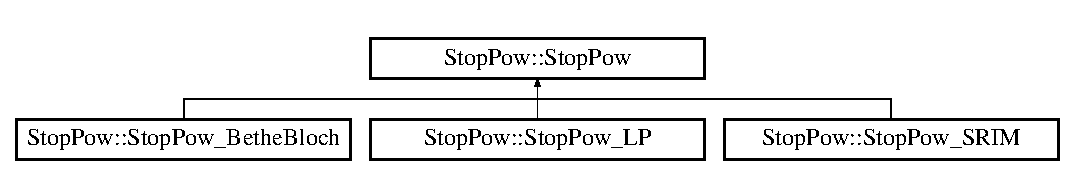
\includegraphics[height=1.914530cm]{class_stop_pow_1_1_stop_pow}
\end{center}
\end{figure}
\subsection*{Public Member Functions}
\begin{DoxyCompactItemize}
\item 
\hyperlink{class_stop_pow_1_1_stop_pow_af65f6d10540615714c734007b06e8fcd}{Stop\-Pow} ()
\item 
\hyperlink{class_stop_pow_1_1_stop_pow_ae497d773c6543a02c1a810a4b705f6a4}{Stop\-Pow} (int set\-\_\-mode)
\item 
float \hyperlink{class_stop_pow_1_1_stop_pow_ad90b7280862a2dca9156b9ebd6992773}{d\-Edx} (float E)
\item 
\hypertarget{class_stop_pow_1_1_stop_pow_af56d6be9eceba6d26eb9f9360f2f14a1}{virtual float {\bfseries d\-Edx\-\_\-\-Me\-V\-\_\-um} (float E)=0}\label{class_stop_pow_1_1_stop_pow_af56d6be9eceba6d26eb9f9360f2f14a1}

\item 
\hypertarget{class_stop_pow_1_1_stop_pow_ae9e6e83483954de70cffbf43f0e2f476}{virtual float {\bfseries d\-Edx\-\_\-\-Me\-V\-\_\-mgcm2} (float E)=0}\label{class_stop_pow_1_1_stop_pow_ae9e6e83483954de70cffbf43f0e2f476}

\item 
\hypertarget{class_stop_pow_1_1_stop_pow_a5f69f88061262399619893c17d956fa2}{virtual float {\bfseries get\-\_\-\-Emin} ()=0}\label{class_stop_pow_1_1_stop_pow_a5f69f88061262399619893c17d956fa2}

\item 
\hypertarget{class_stop_pow_1_1_stop_pow_abef61800dd2420bf2635f152efa73e94}{virtual float {\bfseries get\-\_\-\-Emax} ()=0}\label{class_stop_pow_1_1_stop_pow_abef61800dd2420bf2635f152efa73e94}

\item 
float \hyperlink{class_stop_pow_1_1_stop_pow_ab2bf3d8db19e9c44a79640b1e7835913}{Eout} (float E, float x)
\item 
float \hyperlink{class_stop_pow_1_1_stop_pow_a25d00acea68e066c27219dae57864e9c}{Ein} (float E, float x)
\item 
float \hyperlink{class_stop_pow_1_1_stop_pow_a4596e4cb928d60007b07ff65675ba098}{Thickness} (float E1, float E2)
\item 
float \hyperlink{class_stop_pow_1_1_stop_pow_a92492d239a8a632047d87d447ca8bc69}{get\-\_\-dx} ()
\item 
void \hyperlink{class_stop_pow_1_1_stop_pow_a65260b2b51036a8c7ee82d1156585695}{set\-\_\-dx} (float new\-\_\-dx)
\item 
int \hyperlink{class_stop_pow_1_1_stop_pow_aefe4ad4527d22dde54048cbc94a48a71}{get\-\_\-mode} ()
\item 
void \hyperlink{class_stop_pow_1_1_stop_pow_a661714999f4a47d8a03579d8ef07a172}{set\-\_\-mode} (int new\-\_\-mode)
\end{DoxyCompactItemize}
\subsection*{Static Public Attributes}
\begin{DoxyCompactItemize}
\item 
\hypertarget{class_stop_pow_1_1_stop_pow_a64181f1c265a51d1e404045b8e958438}{static const float {\bfseries D\-E\-F\-A\-U\-L\-T\-\_\-\-D\-X}}\label{class_stop_pow_1_1_stop_pow_a64181f1c265a51d1e404045b8e958438}

\item 
\hypertarget{class_stop_pow_1_1_stop_pow_abf5e1ae5fbd8f4e697b7c0480513650d}{static const float {\bfseries D\-E\-F\-A\-U\-L\-T\-\_\-\-D\-R\-H\-O\-R}}\label{class_stop_pow_1_1_stop_pow_abf5e1ae5fbd8f4e697b7c0480513650d}

\item 
\hypertarget{class_stop_pow_1_1_stop_pow_a58f91fb9fd2229ff96ca593bb83e8991}{static const int {\bfseries M\-O\-D\-E\-\_\-\-L\-E\-N\-G\-T\-H}}\label{class_stop_pow_1_1_stop_pow_a58f91fb9fd2229ff96ca593bb83e8991}

\item 
\hypertarget{class_stop_pow_1_1_stop_pow_af32961a5108b85bb4fa0747cbf4e6398}{static const int {\bfseries M\-O\-D\-E\-\_\-\-R\-H\-O\-R}}\label{class_stop_pow_1_1_stop_pow_af32961a5108b85bb4fa0747cbf4e6398}

\end{DoxyCompactItemize}
\subsection*{Protected Attributes}
\begin{DoxyCompactItemize}
\item 
\hypertarget{class_stop_pow_1_1_stop_pow_a6cf58bdac423b48c9d8b4e8f33da65a9}{float {\bfseries dx}}\label{class_stop_pow_1_1_stop_pow_a6cf58bdac423b48c9d8b4e8f33da65a9}

\item 
\hypertarget{class_stop_pow_1_1_stop_pow_a37d8b949dde8d4eb392f11f3a9cf0272}{int {\bfseries mode}}\label{class_stop_pow_1_1_stop_pow_a37d8b949dde8d4eb392f11f3a9cf0272}

\end{DoxyCompactItemize}


\subsection{Constructor \& Destructor Documentation}
\hypertarget{class_stop_pow_1_1_stop_pow_af65f6d10540615714c734007b06e8fcd}{\index{Stop\-Pow\-::\-Stop\-Pow@{Stop\-Pow\-::\-Stop\-Pow}!Stop\-Pow@{Stop\-Pow}}
\index{Stop\-Pow@{Stop\-Pow}!StopPow::StopPow@{Stop\-Pow\-::\-Stop\-Pow}}
\subsubsection[{Stop\-Pow}]{\setlength{\rightskip}{0pt plus 5cm}Stop\-Pow\-::\-Stop\-Pow\-::\-Stop\-Pow (
\begin{DoxyParamCaption}
{}
\end{DoxyParamCaption}
)}}\label{class_stop_pow_1_1_stop_pow_af65f6d10540615714c734007b06e8fcd}
Simple constructor for the generic class \hypertarget{class_stop_pow_1_1_stop_pow_ae497d773c6543a02c1a810a4b705f6a4}{\index{Stop\-Pow\-::\-Stop\-Pow@{Stop\-Pow\-::\-Stop\-Pow}!Stop\-Pow@{Stop\-Pow}}
\index{Stop\-Pow@{Stop\-Pow}!StopPow::StopPow@{Stop\-Pow\-::\-Stop\-Pow}}
\subsubsection[{Stop\-Pow}]{\setlength{\rightskip}{0pt plus 5cm}Stop\-Pow\-::\-Stop\-Pow\-::\-Stop\-Pow (
\begin{DoxyParamCaption}
\item[{int}]{set\-\_\-mode}
\end{DoxyParamCaption}
)\hspace{0.3cm}{\ttfamily [explicit]}}}\label{class_stop_pow_1_1_stop_pow_ae497d773c6543a02c1a810a4b705f6a4}
Construct a new \hyperlink{class_stop_pow_1_1_stop_pow}{Stop\-Pow} object given a starting mode 
\begin{DoxyParams}{Parameters}
{\em set\-\_\-mode} & the mode you want to use (defined using class constants) \\
\hline
\end{DoxyParams}


\subsection{Member Function Documentation}
\hypertarget{class_stop_pow_1_1_stop_pow_ad90b7280862a2dca9156b9ebd6992773}{\index{Stop\-Pow\-::\-Stop\-Pow@{Stop\-Pow\-::\-Stop\-Pow}!d\-Edx@{d\-Edx}}
\index{d\-Edx@{d\-Edx}!StopPow::StopPow@{Stop\-Pow\-::\-Stop\-Pow}}
\subsubsection[{d\-Edx}]{\setlength{\rightskip}{0pt plus 5cm}float Stop\-Pow\-::\-Stop\-Pow\-::d\-Edx (
\begin{DoxyParamCaption}
\item[{float}]{E}
\end{DoxyParamCaption}
)}}\label{class_stop_pow_1_1_stop_pow_ad90b7280862a2dca9156b9ebd6992773}
Calculate stopping power. Return units depend on mode. 
\begin{DoxyParams}{Parameters}
{\em E} & the particle energy in Me\-V \\
\hline
\end{DoxyParams}
\begin{DoxyReturn}{Returns}
d\-E/dx in Me\-V/um \mbox{[}Me\-V/(mg/cm2)\mbox{]} 
\end{DoxyReturn}

\begin{DoxyExceptions}{Exceptions}
{\em invalid\-\_\-argument} & \\
\hline
\end{DoxyExceptions}
\hypertarget{class_stop_pow_1_1_stop_pow_a25d00acea68e066c27219dae57864e9c}{\index{Stop\-Pow\-::\-Stop\-Pow@{Stop\-Pow\-::\-Stop\-Pow}!Ein@{Ein}}
\index{Ein@{Ein}!StopPow::StopPow@{Stop\-Pow\-::\-Stop\-Pow}}
\subsubsection[{Ein}]{\setlength{\rightskip}{0pt plus 5cm}float Stop\-Pow\-::\-Stop\-Pow\-::\-Ein (
\begin{DoxyParamCaption}
\item[{float}]{E, }
\item[{float}]{x}
\end{DoxyParamCaption}
)}}\label{class_stop_pow_1_1_stop_pow_a25d00acea68e066c27219dae57864e9c}
Get incident energy for a particle. 
\begin{DoxyParams}{Parameters}
{\em E} & the particle energy in Me\-V \\
\hline
{\em x} & thickness of material in um \mbox{[}mg/cm2\mbox{]} \\
\hline
\end{DoxyParams}
\begin{DoxyReturn}{Returns}
initial particle energy in Me\-V 
\end{DoxyReturn}

\begin{DoxyExceptions}{Exceptions}
{\em invalid\-\_\-argument} & \\
\hline
\end{DoxyExceptions}
\hypertarget{class_stop_pow_1_1_stop_pow_ab2bf3d8db19e9c44a79640b1e7835913}{\index{Stop\-Pow\-::\-Stop\-Pow@{Stop\-Pow\-::\-Stop\-Pow}!Eout@{Eout}}
\index{Eout@{Eout}!StopPow::StopPow@{Stop\-Pow\-::\-Stop\-Pow}}
\subsubsection[{Eout}]{\setlength{\rightskip}{0pt plus 5cm}float Stop\-Pow\-::\-Stop\-Pow\-::\-Eout (
\begin{DoxyParamCaption}
\item[{float}]{E, }
\item[{float}]{x}
\end{DoxyParamCaption}
)}}\label{class_stop_pow_1_1_stop_pow_ab2bf3d8db19e9c44a79640b1e7835913}
Get energy downshift for a particle. 
\begin{DoxyParams}{Parameters}
{\em E} & the particle energy in Me\-V \\
\hline
{\em x} & thickness of material in um \mbox{[}mg/cm2\mbox{]} \\
\hline
\end{DoxyParams}
\begin{DoxyReturn}{Returns}
final particle energy in Me\-V 
\end{DoxyReturn}

\begin{DoxyExceptions}{Exceptions}
{\em invalid\-\_\-argument} & \\
\hline
\end{DoxyExceptions}
\hypertarget{class_stop_pow_1_1_stop_pow_a92492d239a8a632047d87d447ca8bc69}{\index{Stop\-Pow\-::\-Stop\-Pow@{Stop\-Pow\-::\-Stop\-Pow}!get\-\_\-dx@{get\-\_\-dx}}
\index{get\-\_\-dx@{get\-\_\-dx}!StopPow::StopPow@{Stop\-Pow\-::\-Stop\-Pow}}
\subsubsection[{get\-\_\-dx}]{\setlength{\rightskip}{0pt plus 5cm}float Stop\-Pow\-::\-Stop\-Pow\-::get\-\_\-dx (
\begin{DoxyParamCaption}
{}
\end{DoxyParamCaption}
)}}\label{class_stop_pow_1_1_stop_pow_a92492d239a8a632047d87d447ca8bc69}
Get the current step sized being used for calculations. \begin{DoxyReturn}{Returns}
dx the step size in um \mbox{[}mg/cm2\mbox{]} 
\end{DoxyReturn}
\hypertarget{class_stop_pow_1_1_stop_pow_aefe4ad4527d22dde54048cbc94a48a71}{\index{Stop\-Pow\-::\-Stop\-Pow@{Stop\-Pow\-::\-Stop\-Pow}!get\-\_\-mode@{get\-\_\-mode}}
\index{get\-\_\-mode@{get\-\_\-mode}!StopPow::StopPow@{Stop\-Pow\-::\-Stop\-Pow}}
\subsubsection[{get\-\_\-mode}]{\setlength{\rightskip}{0pt plus 5cm}int Stop\-Pow\-::\-Stop\-Pow\-::get\-\_\-mode (
\begin{DoxyParamCaption}
{}
\end{DoxyParamCaption}
)}}\label{class_stop_pow_1_1_stop_pow_aefe4ad4527d22dde54048cbc94a48a71}
Get the current mode being used for calculations. \begin{DoxyReturn}{Returns}
mode Either Stop\-Pow.\-M\-O\-D\-E\-\_\-\-L\-E\-N\-G\-T\-H or Stop\-Pow.\-M\-O\-D\-E\-\_\-\-R\-H\-O\-R 
\end{DoxyReturn}
\hypertarget{class_stop_pow_1_1_stop_pow_a65260b2b51036a8c7ee82d1156585695}{\index{Stop\-Pow\-::\-Stop\-Pow@{Stop\-Pow\-::\-Stop\-Pow}!set\-\_\-dx@{set\-\_\-dx}}
\index{set\-\_\-dx@{set\-\_\-dx}!StopPow::StopPow@{Stop\-Pow\-::\-Stop\-Pow}}
\subsubsection[{set\-\_\-dx}]{\setlength{\rightskip}{0pt plus 5cm}void Stop\-Pow\-::\-Stop\-Pow\-::set\-\_\-dx (
\begin{DoxyParamCaption}
\item[{float}]{new\-\_\-dx}
\end{DoxyParamCaption}
)}}\label{class_stop_pow_1_1_stop_pow_a65260b2b51036a8c7ee82d1156585695}
Set the step size for calculations 
\begin{DoxyParams}{Parameters}
{\em new\-\_\-dx} & the new step size to use, in um \mbox{[}mg/cm2\mbox{]} \\
\hline
\end{DoxyParams}

\begin{DoxyExceptions}{Exceptions}
{\em invalid\-\_\-argument} & \\
\hline
\end{DoxyExceptions}
\hypertarget{class_stop_pow_1_1_stop_pow_a661714999f4a47d8a03579d8ef07a172}{\index{Stop\-Pow\-::\-Stop\-Pow@{Stop\-Pow\-::\-Stop\-Pow}!set\-\_\-mode@{set\-\_\-mode}}
\index{set\-\_\-mode@{set\-\_\-mode}!StopPow::StopPow@{Stop\-Pow\-::\-Stop\-Pow}}
\subsubsection[{set\-\_\-mode}]{\setlength{\rightskip}{0pt plus 5cm}void Stop\-Pow\-::\-Stop\-Pow\-::set\-\_\-mode (
\begin{DoxyParamCaption}
\item[{int}]{new\-\_\-mode}
\end{DoxyParamCaption}
)}}\label{class_stop_pow_1_1_stop_pow_a661714999f4a47d8a03579d8ef07a172}
Set the mode for calculations 
\begin{DoxyParams}{Parameters}
{\em new\-\_\-mode} & Either Stop\-Pow.\-M\-O\-D\-E\-\_\-\-L\-E\-N\-G\-T\-H or Stop\-Pow.\-M\-O\-D\-E\-\_\-\-R\-H\-O\-R \\
\hline
\end{DoxyParams}

\begin{DoxyExceptions}{Exceptions}
{\em invalid\-\_\-argument} & \\
\hline
\end{DoxyExceptions}
\hypertarget{class_stop_pow_1_1_stop_pow_a4596e4cb928d60007b07ff65675ba098}{\index{Stop\-Pow\-::\-Stop\-Pow@{Stop\-Pow\-::\-Stop\-Pow}!Thickness@{Thickness}}
\index{Thickness@{Thickness}!StopPow::StopPow@{Stop\-Pow\-::\-Stop\-Pow}}
\subsubsection[{Thickness}]{\setlength{\rightskip}{0pt plus 5cm}float Stop\-Pow\-::\-Stop\-Pow\-::\-Thickness (
\begin{DoxyParamCaption}
\item[{float}]{E1, }
\item[{float}]{E2}
\end{DoxyParamCaption}
)}}\label{class_stop_pow_1_1_stop_pow_a4596e4cb928d60007b07ff65675ba098}
Get thickness of material traversed. 
\begin{DoxyParams}{Parameters}
{\em E1} & the initial particle energy in Me\-V \\
\hline
{\em E2} & the final particle energy in Me\-V \\
\hline
\end{DoxyParams}
\begin{DoxyReturn}{Returns}
material thickness in um \mbox{[}mg/cm2\mbox{]} 
\end{DoxyReturn}

\begin{DoxyExceptions}{Exceptions}
{\em invalid\-\_\-argument} & \\
\hline
\end{DoxyExceptions}


The documentation for this class was generated from the following file\-:\begin{DoxyCompactItemize}
\item 
/\-Users/alex/\-Dropbox/\-Research/\-Code/\-Stop\-Pow/src/Stop\-Pow.\-h\end{DoxyCompactItemize}

\hypertarget{class_stop_pow}{\section{Stop\-Pow Class Reference}
\label{class_stop_pow}\index{Stop\-Pow@{Stop\-Pow}}
}


Generic class for stopping power calculators.  




{\ttfamily \#include $<$Stop\-Pow.\-h$>$}

\subsection*{Public Attributes}
\begin{DoxyCompactItemize}
\item 
\hypertarget{class_stop_pow_a4e2afefafa73a108e367fa714755381a}{const float {\bfseries r0} = 2.\-82e-\/13}\label{class_stop_pow_a4e2afefafa73a108e367fa714755381a}

\item 
\hypertarget{class_stop_pow_a6630f7ecd7d886942178a1d3af07f31b}{const float {\bfseries mec2} = 511}\label{class_stop_pow_a6630f7ecd7d886942178a1d3af07f31b}

\item 
\hypertarget{class_stop_pow_a0bb93119a3657139e678bc0822083974}{const float {\bfseries mpc2} = 9.\-38e5}\label{class_stop_pow_a0bb93119a3657139e678bc0822083974}

\item 
\hypertarget{class_stop_pow_a7ca51e59ba5b8c43a5d969d5b7de1252}{const float {\bfseries c} = 2.\-997e10}\label{class_stop_pow_a7ca51e59ba5b8c43a5d969d5b7de1252}

\item 
\hypertarget{class_stop_pow_ad41f4bc6a9c44c061d07cc60099a99ae}{const float {\bfseries me} = 9.\-109e-\/28}\label{class_stop_pow_ad41f4bc6a9c44c061d07cc60099a99ae}

\item 
\hypertarget{class_stop_pow_aa20c3324505518394c9f182c5df73f8e}{const float {\bfseries mp} = 1.\-6726e-\/24}\label{class_stop_pow_aa20c3324505518394c9f182c5df73f8e}

\item 
\hypertarget{class_stop_pow_a3dc35c0a9d9da229547a1dc05fb5e9cb}{const float {\bfseries k\-B} = 1.\-381e-\/16}\label{class_stop_pow_a3dc35c0a9d9da229547a1dc05fb5e9cb}

\item 
\hypertarget{class_stop_pow_a313a7e44f18ec720ee555b8cc945eaf5}{const float {\bfseries Na} = 6.\-022e23}\label{class_stop_pow_a313a7e44f18ec720ee555b8cc945eaf5}

\item 
\hypertarget{class_stop_pow_a490a4426ad065fc87b8073916a2bfde5}{const float {\bfseries hbar} = 1.\-054e-\/27}\label{class_stop_pow_a490a4426ad065fc87b8073916a2bfde5}

\item 
\hypertarget{class_stop_pow_afc6ea6653f4019089c4f9f5bd533c6dd}{const float {\bfseries e} = 4.\-8e-\/10}\label{class_stop_pow_afc6ea6653f4019089c4f9f5bd533c6dd}

\item 
\hypertarget{class_stop_pow_a7f5bc92566875fc37f39ac91e0c9cf29}{const float {\bfseries ke\-Vto\-K} = 1.\-16e7}\label{class_stop_pow_a7f5bc92566875fc37f39ac91e0c9cf29}

\item 
\hypertarget{class_stop_pow_aca0237f7033276a418eed333c93e4e6f}{const float {\bfseries ke\-Vtoe\-V} = 1.\-602e-\/9}\label{class_stop_pow_aca0237f7033276a418eed333c93e4e6f}

\item 
\hypertarget{class_stop_pow_aaa6917e7a9cef2457c749d7ebac17f45}{const float {\bfseries M\-\_\-\-P\-I} = 3.\-1415926}\label{class_stop_pow_aaa6917e7a9cef2457c749d7ebac17f45}

\end{DoxyCompactItemize}


\subsection{Detailed Description}
Generic class for stopping power calculators. 

In addition to setting the abstract template for stopping power calculators, this also includes several generic methods. The stopping power utilities here can be called as functions of linear distance or areal density. To specify which, the mode must be set correctly.

\begin{DoxyAuthor}{Author}
Alex Zylstra 
\end{DoxyAuthor}
\begin{DoxyDate}{Date}
2013/04/03 
\end{DoxyDate}
\begin{DoxyCopyright}{Copyright}
M\-I\-T / Alex Zylstra 
\end{DoxyCopyright}


The documentation for this class was generated from the following files\-:\begin{DoxyCompactItemize}
\item 
/\-Users/alex/\-Dropbox/\-Research/\-Code/\-Stop\-Pow/src/Stop\-Pow.\-h\item 
/\-Users/alex/\-Dropbox/\-Research/\-Code/\-Stop\-Pow/src/Stop\-Pow\-\_\-\-Constants.\-h\end{DoxyCompactItemize}

\hypertarget{class_stop_pow_1_1_stop_pow___bethe_bloch}{\section{Stop\-Pow\-:\-:Stop\-Pow\-\_\-\-Bethe\-Bloch Class Reference}
\label{class_stop_pow_1_1_stop_pow___bethe_bloch}\index{Stop\-Pow\-::\-Stop\-Pow\-\_\-\-Bethe\-Bloch@{Stop\-Pow\-::\-Stop\-Pow\-\_\-\-Bethe\-Bloch}}
}
Inheritance diagram for Stop\-Pow\-:\-:Stop\-Pow\-\_\-\-Bethe\-Bloch\-:\begin{figure}[H]
\begin{center}
\leavevmode
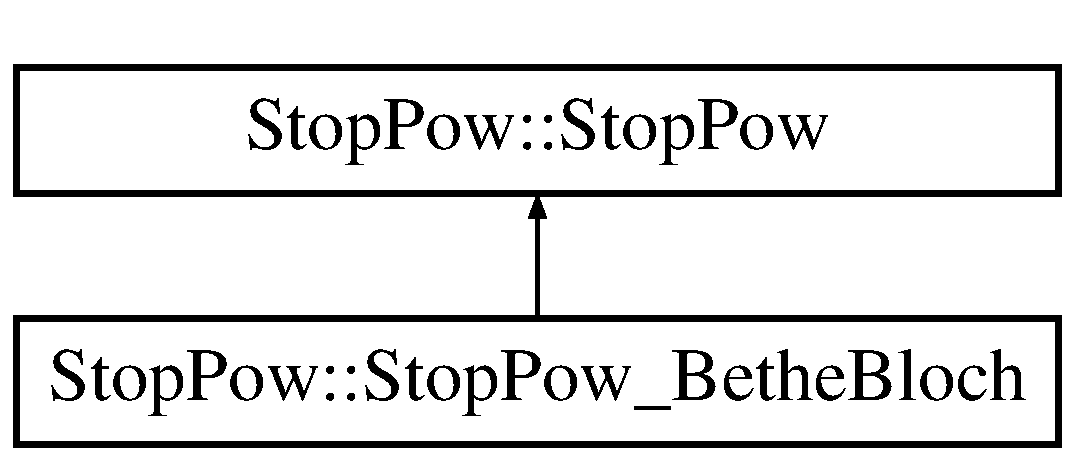
\includegraphics[height=2.000000cm]{class_stop_pow_1_1_stop_pow___bethe_bloch}
\end{center}
\end{figure}
\subsection*{Public Member Functions}
\begin{DoxyCompactItemize}
\item 
\hyperlink{class_stop_pow_1_1_stop_pow___bethe_bloch_ace598f357ec3278c5765377d317944b7}{Stop\-Pow\-\_\-\-Bethe\-Bloch} (float mt, float Zt, std\-::vector$<$ float $>$ mf, std\-::vector$<$ float $>$ Zf, std\-::vector$<$ float $>$ nf)
\item 
float \hyperlink{class_stop_pow_1_1_stop_pow___bethe_bloch_a9c1f3854cc7099c583af66640ffb8223}{d\-Edx\-\_\-\-Me\-V\-\_\-um} (float E)
\item 
float \hyperlink{class_stop_pow_1_1_stop_pow___bethe_bloch_a385fe657e4f3bea2142198e85689c9d6}{d\-Edx\-\_\-\-Me\-V\-\_\-mgcm2} (float E)
\item 
float \hyperlink{class_stop_pow_1_1_stop_pow___bethe_bloch_ae191d6514c38ec7dce0b007f1d63ffef}{get\-\_\-\-Emin} ()
\item 
float \hyperlink{class_stop_pow_1_1_stop_pow___bethe_bloch_a1c554f5107763f3dc37e07776b544f56}{get\-\_\-\-Emax} ()
\end{DoxyCompactItemize}
\subsection*{Additional Inherited Members}


\subsection{Constructor \& Destructor Documentation}
\hypertarget{class_stop_pow_1_1_stop_pow___bethe_bloch_ace598f357ec3278c5765377d317944b7}{\index{Stop\-Pow\-::\-Stop\-Pow\-\_\-\-Bethe\-Bloch@{Stop\-Pow\-::\-Stop\-Pow\-\_\-\-Bethe\-Bloch}!Stop\-Pow\-\_\-\-Bethe\-Bloch@{Stop\-Pow\-\_\-\-Bethe\-Bloch}}
\index{Stop\-Pow\-\_\-\-Bethe\-Bloch@{Stop\-Pow\-\_\-\-Bethe\-Bloch}!StopPow::StopPow_BetheBloch@{Stop\-Pow\-::\-Stop\-Pow\-\_\-\-Bethe\-Bloch}}
\subsubsection[{Stop\-Pow\-\_\-\-Bethe\-Bloch}]{\setlength{\rightskip}{0pt plus 5cm}Stop\-Pow\-::\-Stop\-Pow\-\_\-\-Bethe\-Bloch\-::\-Stop\-Pow\-\_\-\-Bethe\-Bloch (
\begin{DoxyParamCaption}
\item[{float}]{mt, }
\item[{float}]{Zt, }
\item[{std\-::vector$<$ float $>$}]{mf, }
\item[{std\-::vector$<$ float $>$}]{Zf, }
\item[{std\-::vector$<$ float $>$}]{nf}
\end{DoxyParamCaption}
)}}\label{class_stop_pow_1_1_stop_pow___bethe_bloch_ace598f357ec3278c5765377d317944b7}
Initialize the Bethe-\/\-Bloch calculator. 
\begin{DoxyParams}{Parameters}
{\em mt} & the test particle mass in A\-M\-U \\
\hline
{\em Zt} & the test particle in charge (units of e) \\
\hline
{\em mf} & vector containing ordered field particle masses in A\-M\-U \\
\hline
{\em Zt} & vector containing ordered field particle charges in units of e \\
\hline
{\em nf} & vector containing ordered field particle densities in units of 1/cm3 \\
\hline
\end{DoxyParams}

\begin{DoxyExceptions}{Exceptions}
{\em invalid\-\_\-argument} & \\
\hline
\end{DoxyExceptions}


\subsection{Member Function Documentation}
\hypertarget{class_stop_pow_1_1_stop_pow___bethe_bloch_a385fe657e4f3bea2142198e85689c9d6}{\index{Stop\-Pow\-::\-Stop\-Pow\-\_\-\-Bethe\-Bloch@{Stop\-Pow\-::\-Stop\-Pow\-\_\-\-Bethe\-Bloch}!d\-Edx\-\_\-\-Me\-V\-\_\-mgcm2@{d\-Edx\-\_\-\-Me\-V\-\_\-mgcm2}}
\index{d\-Edx\-\_\-\-Me\-V\-\_\-mgcm2@{d\-Edx\-\_\-\-Me\-V\-\_\-mgcm2}!StopPow::StopPow_BetheBloch@{Stop\-Pow\-::\-Stop\-Pow\-\_\-\-Bethe\-Bloch}}
\subsubsection[{d\-Edx\-\_\-\-Me\-V\-\_\-mgcm2}]{\setlength{\rightskip}{0pt plus 5cm}float Stop\-Pow\-::\-Stop\-Pow\-\_\-\-Bethe\-Bloch\-::d\-Edx\-\_\-\-Me\-V\-\_\-mgcm2 (
\begin{DoxyParamCaption}
\item[{float}]{E}
\end{DoxyParamCaption}
)\hspace{0.3cm}{\ttfamily [virtual]}}}\label{class_stop_pow_1_1_stop_pow___bethe_bloch_a385fe657e4f3bea2142198e85689c9d6}
Calculate the total stopping power 
\begin{DoxyParams}{Parameters}
{\em E} & the test particle energy in Me\-V \\
\hline
\end{DoxyParams}
\begin{DoxyReturn}{Returns}
stopping power in units of Me\-V/(mg/cm2) 
\end{DoxyReturn}

\begin{DoxyExceptions}{Exceptions}
{\em invalid\-\_\-argument} & \\
\hline
\end{DoxyExceptions}


Implements \hyperlink{class_stop_pow_1_1_stop_pow}{Stop\-Pow\-::\-Stop\-Pow}.

\hypertarget{class_stop_pow_1_1_stop_pow___bethe_bloch_a9c1f3854cc7099c583af66640ffb8223}{\index{Stop\-Pow\-::\-Stop\-Pow\-\_\-\-Bethe\-Bloch@{Stop\-Pow\-::\-Stop\-Pow\-\_\-\-Bethe\-Bloch}!d\-Edx\-\_\-\-Me\-V\-\_\-um@{d\-Edx\-\_\-\-Me\-V\-\_\-um}}
\index{d\-Edx\-\_\-\-Me\-V\-\_\-um@{d\-Edx\-\_\-\-Me\-V\-\_\-um}!StopPow::StopPow_BetheBloch@{Stop\-Pow\-::\-Stop\-Pow\-\_\-\-Bethe\-Bloch}}
\subsubsection[{d\-Edx\-\_\-\-Me\-V\-\_\-um}]{\setlength{\rightskip}{0pt plus 5cm}float Stop\-Pow\-::\-Stop\-Pow\-\_\-\-Bethe\-Bloch\-::d\-Edx\-\_\-\-Me\-V\-\_\-um (
\begin{DoxyParamCaption}
\item[{float}]{E}
\end{DoxyParamCaption}
)\hspace{0.3cm}{\ttfamily [virtual]}}}\label{class_stop_pow_1_1_stop_pow___bethe_bloch_a9c1f3854cc7099c583af66640ffb8223}
Calculate the total stopping power 
\begin{DoxyParams}{Parameters}
{\em E} & the test particle energy in Me\-V \\
\hline
\end{DoxyParams}
\begin{DoxyReturn}{Returns}
stopping power in units of Me\-V/um 
\end{DoxyReturn}

\begin{DoxyExceptions}{Exceptions}
{\em invalid\-\_\-argument} & \\
\hline
\end{DoxyExceptions}


Implements \hyperlink{class_stop_pow_1_1_stop_pow}{Stop\-Pow\-::\-Stop\-Pow}.

\hypertarget{class_stop_pow_1_1_stop_pow___bethe_bloch_a1c554f5107763f3dc37e07776b544f56}{\index{Stop\-Pow\-::\-Stop\-Pow\-\_\-\-Bethe\-Bloch@{Stop\-Pow\-::\-Stop\-Pow\-\_\-\-Bethe\-Bloch}!get\-\_\-\-Emax@{get\-\_\-\-Emax}}
\index{get\-\_\-\-Emax@{get\-\_\-\-Emax}!StopPow::StopPow_BetheBloch@{Stop\-Pow\-::\-Stop\-Pow\-\_\-\-Bethe\-Bloch}}
\subsubsection[{get\-\_\-\-Emax}]{\setlength{\rightskip}{0pt plus 5cm}float Stop\-Pow\-::\-Stop\-Pow\-\_\-\-Bethe\-Bloch\-::get\-\_\-\-Emax (
\begin{DoxyParamCaption}
{}
\end{DoxyParamCaption}
)\hspace{0.3cm}{\ttfamily [virtual]}}}\label{class_stop_pow_1_1_stop_pow___bethe_bloch_a1c554f5107763f3dc37e07776b544f56}
Get the maximum energy that can be used for d\-E/dx calculations \begin{DoxyReturn}{Returns}
Emax in Me\-V 
\end{DoxyReturn}


Implements \hyperlink{class_stop_pow_1_1_stop_pow}{Stop\-Pow\-::\-Stop\-Pow}.

\hypertarget{class_stop_pow_1_1_stop_pow___bethe_bloch_ae191d6514c38ec7dce0b007f1d63ffef}{\index{Stop\-Pow\-::\-Stop\-Pow\-\_\-\-Bethe\-Bloch@{Stop\-Pow\-::\-Stop\-Pow\-\_\-\-Bethe\-Bloch}!get\-\_\-\-Emin@{get\-\_\-\-Emin}}
\index{get\-\_\-\-Emin@{get\-\_\-\-Emin}!StopPow::StopPow_BetheBloch@{Stop\-Pow\-::\-Stop\-Pow\-\_\-\-Bethe\-Bloch}}
\subsubsection[{get\-\_\-\-Emin}]{\setlength{\rightskip}{0pt plus 5cm}float Stop\-Pow\-::\-Stop\-Pow\-\_\-\-Bethe\-Bloch\-::get\-\_\-\-Emin (
\begin{DoxyParamCaption}
{}
\end{DoxyParamCaption}
)\hspace{0.3cm}{\ttfamily [virtual]}}}\label{class_stop_pow_1_1_stop_pow___bethe_bloch_ae191d6514c38ec7dce0b007f1d63ffef}
Get the minimum energy that can be used for d\-E/dx calculations \begin{DoxyReturn}{Returns}
Emin in Me\-V 
\end{DoxyReturn}


Implements \hyperlink{class_stop_pow_1_1_stop_pow}{Stop\-Pow\-::\-Stop\-Pow}.



The documentation for this class was generated from the following file\-:\begin{DoxyCompactItemize}
\item 
/\-Users/alex/\-Dropbox/\-Research/\-Code/\-Stop\-Pow/src/Stop\-Pow\-\_\-\-Bethe\-Bloch.\-h\end{DoxyCompactItemize}

\hypertarget{class_stop_pow___bethe_bloch}{\section{Stop\-Pow\-\_\-\-Bethe\-Bloch Class Reference}
\label{class_stop_pow___bethe_bloch}\index{Stop\-Pow\-\_\-\-Bethe\-Bloch@{Stop\-Pow\-\_\-\-Bethe\-Bloch}}
}


Calculate Bethe-\/\-Bloch stopping power.  




{\ttfamily \#include $<$Stop\-Pow\-\_\-\-Bethe\-Bloch.\-h$>$}



\subsection{Detailed Description}
Calculate Bethe-\/\-Bloch stopping power. 

Implement a stopping-\/power calculator for arbitrary cold matter, using the simple Bethe-\/\-Bloch theory.

\begin{DoxyAuthor}{Author}
Alex Zylstra 
\end{DoxyAuthor}
\begin{DoxyDate}{Date}
2013/04/03 
\end{DoxyDate}
\begin{DoxyCopyright}{Copyright}
M\-I\-T / Alex Zylstra 
\end{DoxyCopyright}


The documentation for this class was generated from the following file\-:\begin{DoxyCompactItemize}
\item 
/\-Users/alex/\-Dropbox/\-Research/\-Code/\-Stop\-Pow/src/Stop\-Pow\-\_\-\-Bethe\-Bloch.\-h\end{DoxyCompactItemize}

\hypertarget{class_stop_pow___l_p}{\section{Stop\-Pow\-\_\-\-L\-P Class Reference}
\label{class_stop_pow___l_p}\index{Stop\-Pow\-\_\-\-L\-P@{Stop\-Pow\-\_\-\-L\-P}}
}


Calculate Li-\/\-Petrasso stopping power.  




{\ttfamily \#include $<$Stop\-Pow\-\_\-\-L\-P.\-h$>$}

Inheritance diagram for Stop\-Pow\-\_\-\-L\-P\-:\begin{figure}[H]
\begin{center}
\leavevmode
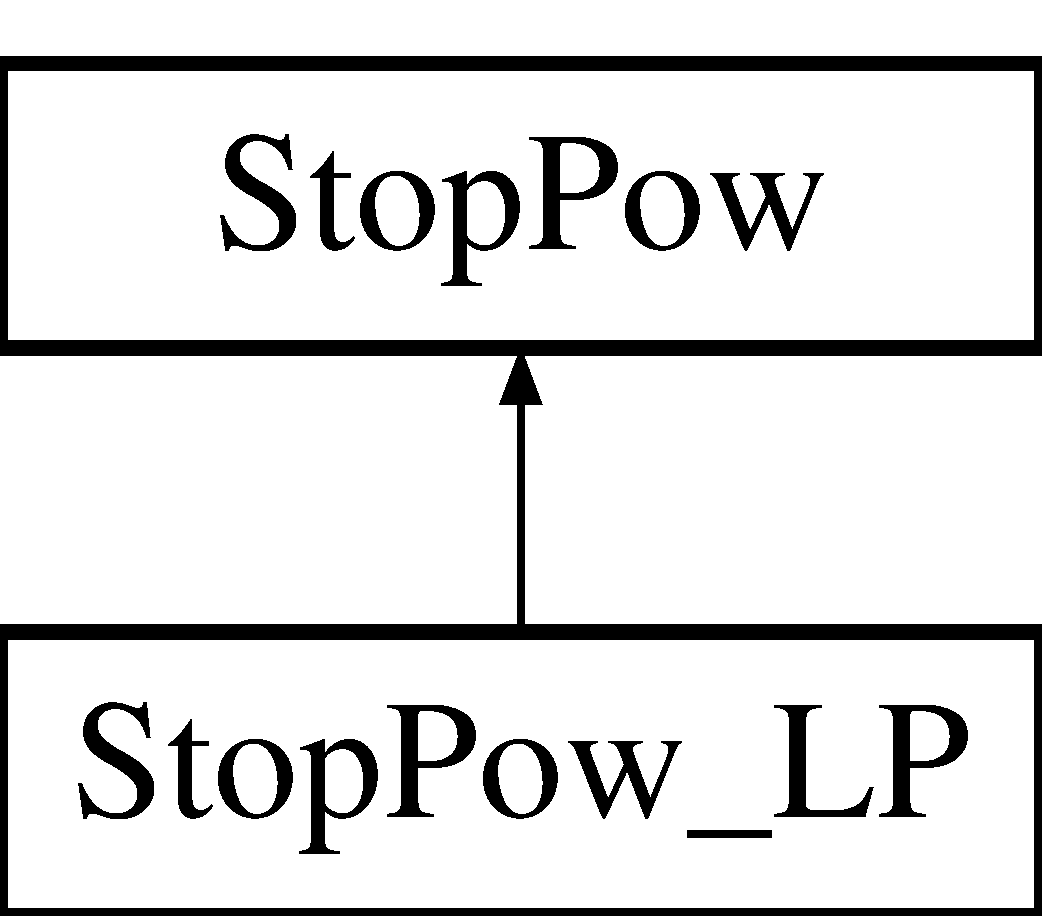
\includegraphics[height=2.000000cm]{class_stop_pow___l_p}
\end{center}
\end{figure}
\subsection*{Public Member Functions}
\begin{DoxyCompactItemize}
\item 
\hyperlink{class_stop_pow___l_p_a342a69be12f73b3d806a60817fa2c5ef}{Stop\-Pow\-\_\-\-L\-P} (float mt, float Zt, vector$<$ float $>$ mf, vector$<$ float $>$ Zf, vector$<$ float $>$ Tf, vector$<$ float $>$ nf)
\item 
float \hyperlink{class_stop_pow___l_p_a0064b2733a7c65d35779d911c8d91cd9}{d\-Edx\-\_\-\-Me\-V\-\_\-um} (float E)
\item 
float \hyperlink{class_stop_pow___l_p_a41a4a36b3a6255a1aed980e127c77af1}{d\-Edx\-\_\-\-Me\-V\-\_\-mgcm2} (float E)
\item 
void \hyperlink{class_stop_pow___l_p_a6681c2fe11c394e0f5515c10db9ef677}{set\-\_\-collective} (bool set)
\end{DoxyCompactItemize}
\subsection*{Additional Inherited Members}


\subsection{Detailed Description}
Calculate Li-\/\-Petrasso stopping power. 

Implement a stopping-\/power calculator for plasma, using the Fokker-\/\-Planck theory described in Li and Petrasso, P\-R\-L 1993.

\begin{DoxyAuthor}{Author}
Alex Zylstra 
\end{DoxyAuthor}
\begin{DoxyDate}{Date}
2013/03/29 
\end{DoxyDate}


\subsection{Constructor \& Destructor Documentation}
\hypertarget{class_stop_pow___l_p_a342a69be12f73b3d806a60817fa2c5ef}{\index{Stop\-Pow\-\_\-\-L\-P@{Stop\-Pow\-\_\-\-L\-P}!Stop\-Pow\-\_\-\-L\-P@{Stop\-Pow\-\_\-\-L\-P}}
\index{Stop\-Pow\-\_\-\-L\-P@{Stop\-Pow\-\_\-\-L\-P}!StopPow_LP@{Stop\-Pow\-\_\-\-L\-P}}
\subsubsection[{Stop\-Pow\-\_\-\-L\-P}]{\setlength{\rightskip}{0pt plus 5cm}Stop\-Pow\-\_\-\-L\-P\-::\-Stop\-Pow\-\_\-\-L\-P (
\begin{DoxyParamCaption}
\item[{float}]{mt, }
\item[{float}]{Zt, }
\item[{vector$<$ float $>$}]{mf, }
\item[{vector$<$ float $>$}]{Zf, }
\item[{vector$<$ float $>$}]{Tf, }
\item[{vector$<$ float $>$}]{nf}
\end{DoxyParamCaption}
)}}\label{class_stop_pow___l_p_a342a69be12f73b3d806a60817fa2c5ef}
Initialize the Li-\/\-Petrasso stopping power. 
\begin{DoxyParams}{Parameters}
{\em mt} & the test particle mass in A\-M\-U \\
\hline
{\em Zt} & the test particle in charge (units of e) \\
\hline
{\em mf} & vector containing ordered field particle masses in A\-M\-U \\
\hline
{\em Zt} & vector containing ordered field particle charges in units of e \\
\hline
{\em Tf} & vector containing ordered field particle temperatures in units of ke\-V \\
\hline
{\em nf} & vector containing ordered field particle densities in units of 1/cm3 \\
\hline
\end{DoxyParams}

\begin{DoxyExceptions}{Exceptions}
{\em invalid\-\_\-argument} & \\
\hline
\end{DoxyExceptions}


\subsection{Member Function Documentation}
\hypertarget{class_stop_pow___l_p_a41a4a36b3a6255a1aed980e127c77af1}{\index{Stop\-Pow\-\_\-\-L\-P@{Stop\-Pow\-\_\-\-L\-P}!d\-Edx\-\_\-\-Me\-V\-\_\-mgcm2@{d\-Edx\-\_\-\-Me\-V\-\_\-mgcm2}}
\index{d\-Edx\-\_\-\-Me\-V\-\_\-mgcm2@{d\-Edx\-\_\-\-Me\-V\-\_\-mgcm2}!StopPow_LP@{Stop\-Pow\-\_\-\-L\-P}}
\subsubsection[{d\-Edx\-\_\-\-Me\-V\-\_\-mgcm2}]{\setlength{\rightskip}{0pt plus 5cm}float Stop\-Pow\-\_\-\-L\-P\-::d\-Edx\-\_\-\-Me\-V\-\_\-mgcm2 (
\begin{DoxyParamCaption}
\item[{float}]{E}
\end{DoxyParamCaption}
)\hspace{0.3cm}{\ttfamily [virtual]}}}\label{class_stop_pow___l_p_a41a4a36b3a6255a1aed980e127c77af1}
Calculate the total stopping power 
\begin{DoxyParams}{Parameters}
{\em E} & the test particle energy in Me\-V \\
\hline
\end{DoxyParams}
\begin{DoxyReturn}{Returns}
stopping power in units of Me\-V/(mg/cm2) 
\end{DoxyReturn}

\begin{DoxyExceptions}{Exceptions}
{\em invalid\-\_\-argument} & \\
\hline
\end{DoxyExceptions}


Implements \hyperlink{class_stop_pow}{Stop\-Pow}.

\hypertarget{class_stop_pow___l_p_a0064b2733a7c65d35779d911c8d91cd9}{\index{Stop\-Pow\-\_\-\-L\-P@{Stop\-Pow\-\_\-\-L\-P}!d\-Edx\-\_\-\-Me\-V\-\_\-um@{d\-Edx\-\_\-\-Me\-V\-\_\-um}}
\index{d\-Edx\-\_\-\-Me\-V\-\_\-um@{d\-Edx\-\_\-\-Me\-V\-\_\-um}!StopPow_LP@{Stop\-Pow\-\_\-\-L\-P}}
\subsubsection[{d\-Edx\-\_\-\-Me\-V\-\_\-um}]{\setlength{\rightskip}{0pt plus 5cm}float Stop\-Pow\-\_\-\-L\-P\-::d\-Edx\-\_\-\-Me\-V\-\_\-um (
\begin{DoxyParamCaption}
\item[{float}]{E}
\end{DoxyParamCaption}
)\hspace{0.3cm}{\ttfamily [virtual]}}}\label{class_stop_pow___l_p_a0064b2733a7c65d35779d911c8d91cd9}
Calculate the total stopping power 
\begin{DoxyParams}{Parameters}
{\em E} & the test particle energy in Me\-V \\
\hline
\end{DoxyParams}
\begin{DoxyReturn}{Returns}
stopping power in units of Me\-V/um 
\end{DoxyReturn}

\begin{DoxyExceptions}{Exceptions}
{\em invalid\-\_\-argument} & \\
\hline
\end{DoxyExceptions}


Implements \hyperlink{class_stop_pow}{Stop\-Pow}.

\hypertarget{class_stop_pow___l_p_a6681c2fe11c394e0f5515c10db9ef677}{\index{Stop\-Pow\-\_\-\-L\-P@{Stop\-Pow\-\_\-\-L\-P}!set\-\_\-collective@{set\-\_\-collective}}
\index{set\-\_\-collective@{set\-\_\-collective}!StopPow_LP@{Stop\-Pow\-\_\-\-L\-P}}
\subsubsection[{set\-\_\-collective}]{\setlength{\rightskip}{0pt plus 5cm}void Stop\-Pow\-\_\-\-L\-P\-::set\-\_\-collective (
\begin{DoxyParamCaption}
\item[{bool}]{set}
\end{DoxyParamCaption}
)}}\label{class_stop_pow___l_p_a6681c2fe11c394e0f5515c10db9ef677}
Turn collective effects on or off. 
\begin{DoxyParams}{Parameters}
{\em set} & if you want to use collective effects \\
\hline
\end{DoxyParams}


The documentation for this class was generated from the following file\-:\begin{DoxyCompactItemize}
\item 
/\-Users/alex/\-Dropbox/\-Research/workspace/\-Stop\-Pow/src/Stop\-Pow\-\_\-\-L\-P.\-h\end{DoxyCompactItemize}

\hypertarget{class_stop_pow_1_1_stop_pow___l_p}{\section{Stop\-Pow\-:\-:Stop\-Pow\-\_\-\-L\-P Class Reference}
\label{class_stop_pow_1_1_stop_pow___l_p}\index{Stop\-Pow\-::\-Stop\-Pow\-\_\-\-L\-P@{Stop\-Pow\-::\-Stop\-Pow\-\_\-\-L\-P}}
}
Inheritance diagram for Stop\-Pow\-:\-:Stop\-Pow\-\_\-\-L\-P\-:\begin{figure}[H]
\begin{center}
\leavevmode
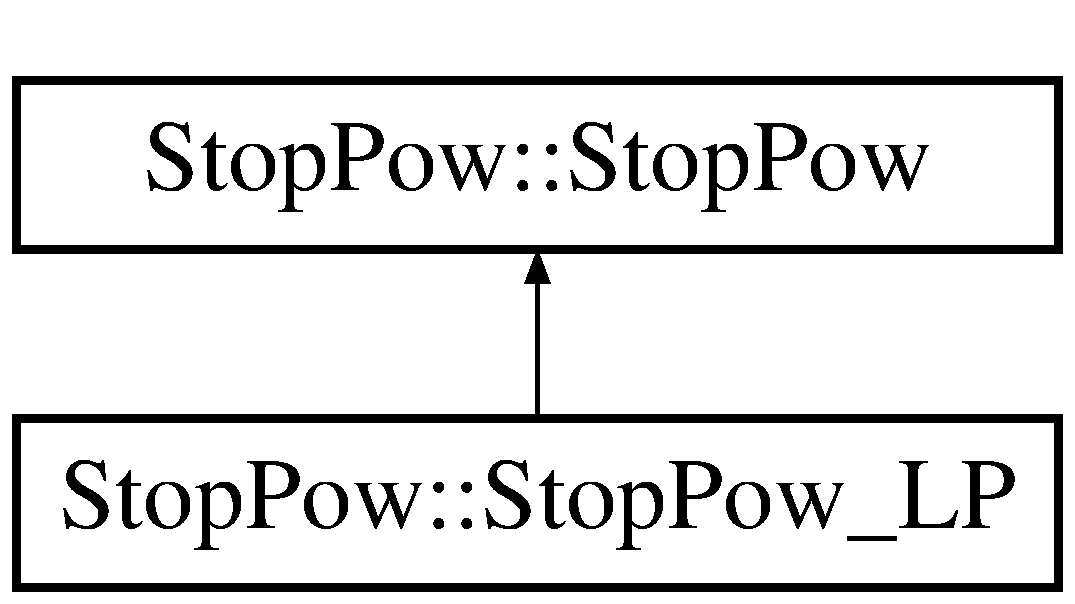
\includegraphics[height=2.000000cm]{class_stop_pow_1_1_stop_pow___l_p}
\end{center}
\end{figure}
\subsection*{Public Member Functions}
\begin{DoxyCompactItemize}
\item 
\hyperlink{class_stop_pow_1_1_stop_pow___l_p_a98c19537a4e112bbd9d062fbfedabf97}{Stop\-Pow\-\_\-\-L\-P} (float mt, float Zt, std\-::vector$<$ float $>$ mf, std\-::vector$<$ float $>$ Zf, std\-::vector$<$ float $>$ Tf, std\-::vector$<$ float $>$ nf)
\item 
float \hyperlink{class_stop_pow_1_1_stop_pow___l_p_af46e3156b2f8ef219649201f0bdd1d1a}{d\-Edx\-\_\-\-Me\-V\-\_\-um} (float E)
\item 
float \hyperlink{class_stop_pow_1_1_stop_pow___l_p_a619b9737b0e2139410c1df6e65781a3b}{d\-Edx\-\_\-\-Me\-V\-\_\-mgcm2} (float E)
\item 
void \hyperlink{class_stop_pow_1_1_stop_pow___l_p_adac0e31284a7a2578f74c671fd0f976a}{set\-\_\-collective} (bool set)
\item 
float \hyperlink{class_stop_pow_1_1_stop_pow___l_p_a810b738fd1addec164711d712865a030}{get\-\_\-\-Emin} ()
\item 
float \hyperlink{class_stop_pow_1_1_stop_pow___l_p_af665f7606e35db7c0c696dda07e2e623}{get\-\_\-\-Emax} ()
\end{DoxyCompactItemize}
\subsection*{Additional Inherited Members}


\subsection{Constructor \& Destructor Documentation}
\hypertarget{class_stop_pow_1_1_stop_pow___l_p_a98c19537a4e112bbd9d062fbfedabf97}{\index{Stop\-Pow\-::\-Stop\-Pow\-\_\-\-L\-P@{Stop\-Pow\-::\-Stop\-Pow\-\_\-\-L\-P}!Stop\-Pow\-\_\-\-L\-P@{Stop\-Pow\-\_\-\-L\-P}}
\index{Stop\-Pow\-\_\-\-L\-P@{Stop\-Pow\-\_\-\-L\-P}!StopPow::StopPow_LP@{Stop\-Pow\-::\-Stop\-Pow\-\_\-\-L\-P}}
\subsubsection[{Stop\-Pow\-\_\-\-L\-P}]{\setlength{\rightskip}{0pt plus 5cm}Stop\-Pow\-::\-Stop\-Pow\-\_\-\-L\-P\-::\-Stop\-Pow\-\_\-\-L\-P (
\begin{DoxyParamCaption}
\item[{float}]{mt, }
\item[{float}]{Zt, }
\item[{std\-::vector$<$ float $>$}]{mf, }
\item[{std\-::vector$<$ float $>$}]{Zf, }
\item[{std\-::vector$<$ float $>$}]{Tf, }
\item[{std\-::vector$<$ float $>$}]{nf}
\end{DoxyParamCaption}
)}}\label{class_stop_pow_1_1_stop_pow___l_p_a98c19537a4e112bbd9d062fbfedabf97}
Initialize the Li-\/\-Petrasso stopping power. 
\begin{DoxyParams}{Parameters}
{\em mt} & the test particle mass in A\-M\-U \\
\hline
{\em Zt} & the test particle in charge (units of e) \\
\hline
{\em mf} & vector containing ordered field particle masses in A\-M\-U \\
\hline
{\em Zt} & vector containing ordered field particle charges in units of e \\
\hline
{\em Tf} & vector containing ordered field particle temperatures in units of ke\-V \\
\hline
{\em nf} & vector containing ordered field particle densities in units of 1/cm3 \\
\hline
\end{DoxyParams}

\begin{DoxyExceptions}{Exceptions}
{\em invalid\-\_\-argument} & \\
\hline
\end{DoxyExceptions}


\subsection{Member Function Documentation}
\hypertarget{class_stop_pow_1_1_stop_pow___l_p_a619b9737b0e2139410c1df6e65781a3b}{\index{Stop\-Pow\-::\-Stop\-Pow\-\_\-\-L\-P@{Stop\-Pow\-::\-Stop\-Pow\-\_\-\-L\-P}!d\-Edx\-\_\-\-Me\-V\-\_\-mgcm2@{d\-Edx\-\_\-\-Me\-V\-\_\-mgcm2}}
\index{d\-Edx\-\_\-\-Me\-V\-\_\-mgcm2@{d\-Edx\-\_\-\-Me\-V\-\_\-mgcm2}!StopPow::StopPow_LP@{Stop\-Pow\-::\-Stop\-Pow\-\_\-\-L\-P}}
\subsubsection[{d\-Edx\-\_\-\-Me\-V\-\_\-mgcm2}]{\setlength{\rightskip}{0pt plus 5cm}float Stop\-Pow\-::\-Stop\-Pow\-\_\-\-L\-P\-::d\-Edx\-\_\-\-Me\-V\-\_\-mgcm2 (
\begin{DoxyParamCaption}
\item[{float}]{E}
\end{DoxyParamCaption}
)\hspace{0.3cm}{\ttfamily [virtual]}}}\label{class_stop_pow_1_1_stop_pow___l_p_a619b9737b0e2139410c1df6e65781a3b}
Calculate the total stopping power 
\begin{DoxyParams}{Parameters}
{\em E} & the test particle energy in Me\-V \\
\hline
\end{DoxyParams}
\begin{DoxyReturn}{Returns}
stopping power in units of Me\-V/(mg/cm2) 
\end{DoxyReturn}

\begin{DoxyExceptions}{Exceptions}
{\em invalid\-\_\-argument} & \\
\hline
\end{DoxyExceptions}


Implements \hyperlink{class_stop_pow_1_1_stop_pow}{Stop\-Pow\-::\-Stop\-Pow}.

\hypertarget{class_stop_pow_1_1_stop_pow___l_p_af46e3156b2f8ef219649201f0bdd1d1a}{\index{Stop\-Pow\-::\-Stop\-Pow\-\_\-\-L\-P@{Stop\-Pow\-::\-Stop\-Pow\-\_\-\-L\-P}!d\-Edx\-\_\-\-Me\-V\-\_\-um@{d\-Edx\-\_\-\-Me\-V\-\_\-um}}
\index{d\-Edx\-\_\-\-Me\-V\-\_\-um@{d\-Edx\-\_\-\-Me\-V\-\_\-um}!StopPow::StopPow_LP@{Stop\-Pow\-::\-Stop\-Pow\-\_\-\-L\-P}}
\subsubsection[{d\-Edx\-\_\-\-Me\-V\-\_\-um}]{\setlength{\rightskip}{0pt plus 5cm}float Stop\-Pow\-::\-Stop\-Pow\-\_\-\-L\-P\-::d\-Edx\-\_\-\-Me\-V\-\_\-um (
\begin{DoxyParamCaption}
\item[{float}]{E}
\end{DoxyParamCaption}
)\hspace{0.3cm}{\ttfamily [virtual]}}}\label{class_stop_pow_1_1_stop_pow___l_p_af46e3156b2f8ef219649201f0bdd1d1a}
Calculate the total stopping power 
\begin{DoxyParams}{Parameters}
{\em E} & the test particle energy in Me\-V \\
\hline
\end{DoxyParams}
\begin{DoxyReturn}{Returns}
stopping power in units of Me\-V/um 
\end{DoxyReturn}

\begin{DoxyExceptions}{Exceptions}
{\em invalid\-\_\-argument} & \\
\hline
\end{DoxyExceptions}


Implements \hyperlink{class_stop_pow_1_1_stop_pow}{Stop\-Pow\-::\-Stop\-Pow}.

\hypertarget{class_stop_pow_1_1_stop_pow___l_p_af665f7606e35db7c0c696dda07e2e623}{\index{Stop\-Pow\-::\-Stop\-Pow\-\_\-\-L\-P@{Stop\-Pow\-::\-Stop\-Pow\-\_\-\-L\-P}!get\-\_\-\-Emax@{get\-\_\-\-Emax}}
\index{get\-\_\-\-Emax@{get\-\_\-\-Emax}!StopPow::StopPow_LP@{Stop\-Pow\-::\-Stop\-Pow\-\_\-\-L\-P}}
\subsubsection[{get\-\_\-\-Emax}]{\setlength{\rightskip}{0pt plus 5cm}float Stop\-Pow\-::\-Stop\-Pow\-\_\-\-L\-P\-::get\-\_\-\-Emax (
\begin{DoxyParamCaption}
{}
\end{DoxyParamCaption}
)\hspace{0.3cm}{\ttfamily [virtual]}}}\label{class_stop_pow_1_1_stop_pow___l_p_af665f7606e35db7c0c696dda07e2e623}
Get the maximum energy that can be used for d\-E/dx calculations \begin{DoxyReturn}{Returns}
Emax in Me\-V 
\end{DoxyReturn}


Implements \hyperlink{class_stop_pow_1_1_stop_pow}{Stop\-Pow\-::\-Stop\-Pow}.

\hypertarget{class_stop_pow_1_1_stop_pow___l_p_a810b738fd1addec164711d712865a030}{\index{Stop\-Pow\-::\-Stop\-Pow\-\_\-\-L\-P@{Stop\-Pow\-::\-Stop\-Pow\-\_\-\-L\-P}!get\-\_\-\-Emin@{get\-\_\-\-Emin}}
\index{get\-\_\-\-Emin@{get\-\_\-\-Emin}!StopPow::StopPow_LP@{Stop\-Pow\-::\-Stop\-Pow\-\_\-\-L\-P}}
\subsubsection[{get\-\_\-\-Emin}]{\setlength{\rightskip}{0pt plus 5cm}float Stop\-Pow\-::\-Stop\-Pow\-\_\-\-L\-P\-::get\-\_\-\-Emin (
\begin{DoxyParamCaption}
{}
\end{DoxyParamCaption}
)\hspace{0.3cm}{\ttfamily [virtual]}}}\label{class_stop_pow_1_1_stop_pow___l_p_a810b738fd1addec164711d712865a030}
Get the minimum energy that can be used for d\-E/dx calculations \begin{DoxyReturn}{Returns}
Emin in Me\-V 
\end{DoxyReturn}


Implements \hyperlink{class_stop_pow_1_1_stop_pow}{Stop\-Pow\-::\-Stop\-Pow}.

\hypertarget{class_stop_pow_1_1_stop_pow___l_p_adac0e31284a7a2578f74c671fd0f976a}{\index{Stop\-Pow\-::\-Stop\-Pow\-\_\-\-L\-P@{Stop\-Pow\-::\-Stop\-Pow\-\_\-\-L\-P}!set\-\_\-collective@{set\-\_\-collective}}
\index{set\-\_\-collective@{set\-\_\-collective}!StopPow::StopPow_LP@{Stop\-Pow\-::\-Stop\-Pow\-\_\-\-L\-P}}
\subsubsection[{set\-\_\-collective}]{\setlength{\rightskip}{0pt plus 5cm}void Stop\-Pow\-::\-Stop\-Pow\-\_\-\-L\-P\-::set\-\_\-collective (
\begin{DoxyParamCaption}
\item[{bool}]{set}
\end{DoxyParamCaption}
)}}\label{class_stop_pow_1_1_stop_pow___l_p_adac0e31284a7a2578f74c671fd0f976a}
Turn collective effects on or off. 
\begin{DoxyParams}{Parameters}
{\em set} & if you want to use collective effects \\
\hline
\end{DoxyParams}


The documentation for this class was generated from the following file\-:\begin{DoxyCompactItemize}
\item 
/\-Users/alex/\-Dropbox/\-Research/\-Code/\-Stop\-Pow/src/Stop\-Pow\-\_\-\-L\-P.\-h\end{DoxyCompactItemize}

\hypertarget{class_stop_pow_1_1_stop_pow___s_r_i_m}{\section{Stop\-Pow\-:\-:Stop\-Pow\-\_\-\-S\-R\-I\-M Class Reference}
\label{class_stop_pow_1_1_stop_pow___s_r_i_m}\index{Stop\-Pow\-::\-Stop\-Pow\-\_\-\-S\-R\-I\-M@{Stop\-Pow\-::\-Stop\-Pow\-\_\-\-S\-R\-I\-M}}
}
Inheritance diagram for Stop\-Pow\-:\-:Stop\-Pow\-\_\-\-S\-R\-I\-M\-:\begin{figure}[H]
\begin{center}
\leavevmode
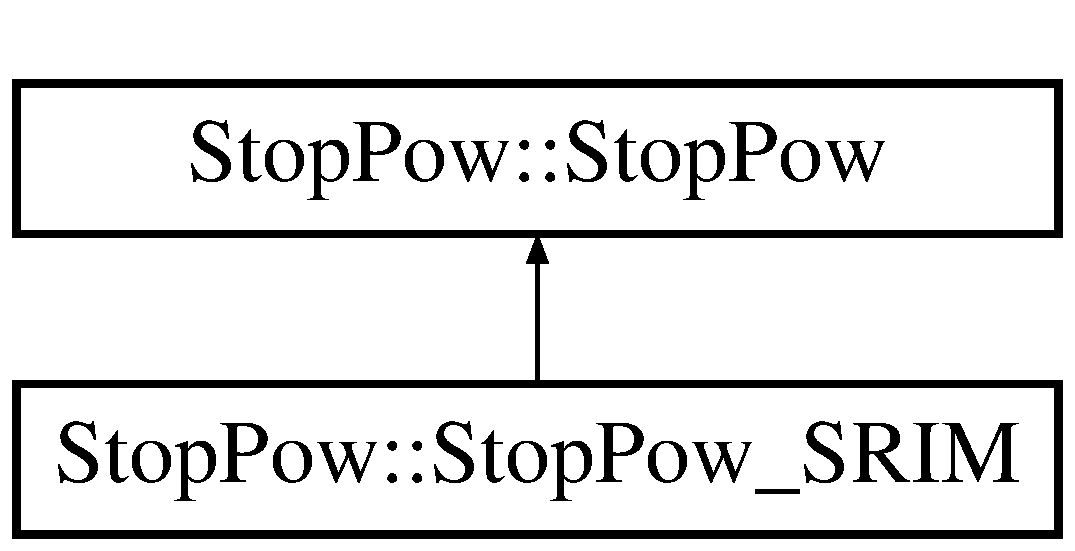
\includegraphics[height=2.000000cm]{class_stop_pow_1_1_stop_pow___s_r_i_m}
\end{center}
\end{figure}
\subsection*{Public Member Functions}
\begin{DoxyCompactItemize}
\item 
\hyperlink{class_stop_pow_1_1_stop_pow___s_r_i_m_aa94b3135a266b128cef16b1f42fca53b}{Stop\-Pow\-\_\-\-S\-R\-I\-M} (std\-::string fname)
\item 
\hyperlink{class_stop_pow_1_1_stop_pow___s_r_i_m_ae4e2b3573df4cac0732b30dbd833fa71}{$\sim$\-Stop\-Pow\-\_\-\-S\-R\-I\-M} ()
\item 
float \hyperlink{class_stop_pow_1_1_stop_pow___s_r_i_m_aaf36060614c8e268d2a4a4db4b77a44d}{d\-Edx\-\_\-\-Me\-V\-\_\-um} (float E)
\item 
float \hyperlink{class_stop_pow_1_1_stop_pow___s_r_i_m_a303d20db094642491b861a07f05c48b6}{d\-Edx\-\_\-\-Me\-V\-\_\-mgcm2} (float E)
\item 
float \hyperlink{class_stop_pow_1_1_stop_pow___s_r_i_m_aedd811155859225354c8d64431f02c4f}{get\-\_\-\-Emin} ()
\item 
float \hyperlink{class_stop_pow_1_1_stop_pow___s_r_i_m_a98bb557b88bf5a9d09cd3d718da36c1f}{get\-\_\-\-Emax} ()
\end{DoxyCompactItemize}
\subsection*{Additional Inherited Members}


\subsection{Constructor \& Destructor Documentation}
\hypertarget{class_stop_pow_1_1_stop_pow___s_r_i_m_aa94b3135a266b128cef16b1f42fca53b}{\index{Stop\-Pow\-::\-Stop\-Pow\-\_\-\-S\-R\-I\-M@{Stop\-Pow\-::\-Stop\-Pow\-\_\-\-S\-R\-I\-M}!Stop\-Pow\-\_\-\-S\-R\-I\-M@{Stop\-Pow\-\_\-\-S\-R\-I\-M}}
\index{Stop\-Pow\-\_\-\-S\-R\-I\-M@{Stop\-Pow\-\_\-\-S\-R\-I\-M}!StopPow::StopPow_SRIM@{Stop\-Pow\-::\-Stop\-Pow\-\_\-\-S\-R\-I\-M}}
\subsubsection[{Stop\-Pow\-\_\-\-S\-R\-I\-M}]{\setlength{\rightskip}{0pt plus 5cm}Stop\-Pow\-::\-Stop\-Pow\-\_\-\-S\-R\-I\-M\-::\-Stop\-Pow\-\_\-\-S\-R\-I\-M (
\begin{DoxyParamCaption}
\item[{std\-::string}]{fname}
\end{DoxyParamCaption}
)\hspace{0.3cm}{\ttfamily [explicit]}}}\label{class_stop_pow_1_1_stop_pow___s_r_i_m_aa94b3135a266b128cef16b1f42fca53b}
Constructor for S\-R\-I\-M object. Data file must be in standard S\-R\-I\-M format. 
\begin{DoxyParams}{Parameters}
{\em fname} & file name (or relative path) for the data \\
\hline
\end{DoxyParams}

\begin{DoxyExceptions}{Exceptions}
{\em ios\-\_\-base\-::failure} & \\
\hline
\end{DoxyExceptions}
\hypertarget{class_stop_pow_1_1_stop_pow___s_r_i_m_ae4e2b3573df4cac0732b30dbd833fa71}{\index{Stop\-Pow\-::\-Stop\-Pow\-\_\-\-S\-R\-I\-M@{Stop\-Pow\-::\-Stop\-Pow\-\_\-\-S\-R\-I\-M}!$\sim$\-Stop\-Pow\-\_\-\-S\-R\-I\-M@{$\sim$\-Stop\-Pow\-\_\-\-S\-R\-I\-M}}
\index{$\sim$\-Stop\-Pow\-\_\-\-S\-R\-I\-M@{$\sim$\-Stop\-Pow\-\_\-\-S\-R\-I\-M}!StopPow::StopPow_SRIM@{Stop\-Pow\-::\-Stop\-Pow\-\_\-\-S\-R\-I\-M}}
\subsubsection[{$\sim$\-Stop\-Pow\-\_\-\-S\-R\-I\-M}]{\setlength{\rightskip}{0pt plus 5cm}Stop\-Pow\-::\-Stop\-Pow\-\_\-\-S\-R\-I\-M\-::$\sim$\-Stop\-Pow\-\_\-\-S\-R\-I\-M (
\begin{DoxyParamCaption}
{}
\end{DoxyParamCaption}
)}}\label{class_stop_pow_1_1_stop_pow___s_r_i_m_ae4e2b3573df4cac0732b30dbd833fa71}
Destructor 

\subsection{Member Function Documentation}
\hypertarget{class_stop_pow_1_1_stop_pow___s_r_i_m_a303d20db094642491b861a07f05c48b6}{\index{Stop\-Pow\-::\-Stop\-Pow\-\_\-\-S\-R\-I\-M@{Stop\-Pow\-::\-Stop\-Pow\-\_\-\-S\-R\-I\-M}!d\-Edx\-\_\-\-Me\-V\-\_\-mgcm2@{d\-Edx\-\_\-\-Me\-V\-\_\-mgcm2}}
\index{d\-Edx\-\_\-\-Me\-V\-\_\-mgcm2@{d\-Edx\-\_\-\-Me\-V\-\_\-mgcm2}!StopPow::StopPow_SRIM@{Stop\-Pow\-::\-Stop\-Pow\-\_\-\-S\-R\-I\-M}}
\subsubsection[{d\-Edx\-\_\-\-Me\-V\-\_\-mgcm2}]{\setlength{\rightskip}{0pt plus 5cm}float Stop\-Pow\-::\-Stop\-Pow\-\_\-\-S\-R\-I\-M\-::d\-Edx\-\_\-\-Me\-V\-\_\-mgcm2 (
\begin{DoxyParamCaption}
\item[{float}]{E}
\end{DoxyParamCaption}
)\hspace{0.3cm}{\ttfamily [virtual]}}}\label{class_stop_pow_1_1_stop_pow___s_r_i_m_a303d20db094642491b861a07f05c48b6}
Get stopping power from the data. 
\begin{DoxyParams}{Parameters}
{\em E} & the particle energy in Me\-V \\
\hline
\end{DoxyParams}
\begin{DoxyReturn}{Returns}
d\-E/dx in Me\-V/(mg/cm2) 
\end{DoxyReturn}

\begin{DoxyExceptions}{Exceptions}
{\em invalid\-\_\-argument} & \\
\hline
\end{DoxyExceptions}


Implements \hyperlink{class_stop_pow_1_1_stop_pow}{Stop\-Pow\-::\-Stop\-Pow}.

\hypertarget{class_stop_pow_1_1_stop_pow___s_r_i_m_aaf36060614c8e268d2a4a4db4b77a44d}{\index{Stop\-Pow\-::\-Stop\-Pow\-\_\-\-S\-R\-I\-M@{Stop\-Pow\-::\-Stop\-Pow\-\_\-\-S\-R\-I\-M}!d\-Edx\-\_\-\-Me\-V\-\_\-um@{d\-Edx\-\_\-\-Me\-V\-\_\-um}}
\index{d\-Edx\-\_\-\-Me\-V\-\_\-um@{d\-Edx\-\_\-\-Me\-V\-\_\-um}!StopPow::StopPow_SRIM@{Stop\-Pow\-::\-Stop\-Pow\-\_\-\-S\-R\-I\-M}}
\subsubsection[{d\-Edx\-\_\-\-Me\-V\-\_\-um}]{\setlength{\rightskip}{0pt plus 5cm}float Stop\-Pow\-::\-Stop\-Pow\-\_\-\-S\-R\-I\-M\-::d\-Edx\-\_\-\-Me\-V\-\_\-um (
\begin{DoxyParamCaption}
\item[{float}]{E}
\end{DoxyParamCaption}
)\hspace{0.3cm}{\ttfamily [virtual]}}}\label{class_stop_pow_1_1_stop_pow___s_r_i_m_aaf36060614c8e268d2a4a4db4b77a44d}
Get stopping power from the data. 
\begin{DoxyParams}{Parameters}
{\em E} & the particle energy in Me\-V \\
\hline
\end{DoxyParams}
\begin{DoxyReturn}{Returns}
d\-E/dx in Me\-V/um 
\end{DoxyReturn}

\begin{DoxyExceptions}{Exceptions}
{\em invalid\-\_\-argument} & \\
\hline
\end{DoxyExceptions}


Implements \hyperlink{class_stop_pow_1_1_stop_pow}{Stop\-Pow\-::\-Stop\-Pow}.

\hypertarget{class_stop_pow_1_1_stop_pow___s_r_i_m_a98bb557b88bf5a9d09cd3d718da36c1f}{\index{Stop\-Pow\-::\-Stop\-Pow\-\_\-\-S\-R\-I\-M@{Stop\-Pow\-::\-Stop\-Pow\-\_\-\-S\-R\-I\-M}!get\-\_\-\-Emax@{get\-\_\-\-Emax}}
\index{get\-\_\-\-Emax@{get\-\_\-\-Emax}!StopPow::StopPow_SRIM@{Stop\-Pow\-::\-Stop\-Pow\-\_\-\-S\-R\-I\-M}}
\subsubsection[{get\-\_\-\-Emax}]{\setlength{\rightskip}{0pt plus 5cm}float Stop\-Pow\-::\-Stop\-Pow\-\_\-\-S\-R\-I\-M\-::get\-\_\-\-Emax (
\begin{DoxyParamCaption}
{}
\end{DoxyParamCaption}
)\hspace{0.3cm}{\ttfamily [virtual]}}}\label{class_stop_pow_1_1_stop_pow___s_r_i_m_a98bb557b88bf5a9d09cd3d718da36c1f}
Get the maximum energy that can be used for d\-E/dx calculations \begin{DoxyReturn}{Returns}
Emax in Me\-V 
\end{DoxyReturn}


Implements \hyperlink{class_stop_pow_1_1_stop_pow}{Stop\-Pow\-::\-Stop\-Pow}.

\hypertarget{class_stop_pow_1_1_stop_pow___s_r_i_m_aedd811155859225354c8d64431f02c4f}{\index{Stop\-Pow\-::\-Stop\-Pow\-\_\-\-S\-R\-I\-M@{Stop\-Pow\-::\-Stop\-Pow\-\_\-\-S\-R\-I\-M}!get\-\_\-\-Emin@{get\-\_\-\-Emin}}
\index{get\-\_\-\-Emin@{get\-\_\-\-Emin}!StopPow::StopPow_SRIM@{Stop\-Pow\-::\-Stop\-Pow\-\_\-\-S\-R\-I\-M}}
\subsubsection[{get\-\_\-\-Emin}]{\setlength{\rightskip}{0pt plus 5cm}float Stop\-Pow\-::\-Stop\-Pow\-\_\-\-S\-R\-I\-M\-::get\-\_\-\-Emin (
\begin{DoxyParamCaption}
{}
\end{DoxyParamCaption}
)\hspace{0.3cm}{\ttfamily [virtual]}}}\label{class_stop_pow_1_1_stop_pow___s_r_i_m_aedd811155859225354c8d64431f02c4f}
Get the minimum energy that can be used for d\-E/dx calculations \begin{DoxyReturn}{Returns}
Emin in Me\-V 
\end{DoxyReturn}


Implements \hyperlink{class_stop_pow_1_1_stop_pow}{Stop\-Pow\-::\-Stop\-Pow}.



The documentation for this class was generated from the following file\-:\begin{DoxyCompactItemize}
\item 
/\-Users/alex/\-Dropbox/\-Research/\-Code/\-Stop\-Pow/src/Stop\-Pow\-\_\-\-S\-R\-I\-M.\-h\end{DoxyCompactItemize}

\hypertarget{class_stop_pow___s_r_i_m}{\section{Stop\-Pow\-\_\-\-S\-R\-I\-M Class Reference}
\label{class_stop_pow___s_r_i_m}\index{Stop\-Pow\-\_\-\-S\-R\-I\-M@{Stop\-Pow\-\_\-\-S\-R\-I\-M}}
}


Cold-\/matter tabulated stopping.  




{\ttfamily \#include $<$Stop\-Pow\-\_\-\-S\-R\-I\-M.\-h$>$}

Inheritance diagram for Stop\-Pow\-\_\-\-S\-R\-I\-M\-:\begin{figure}[H]
\begin{center}
\leavevmode
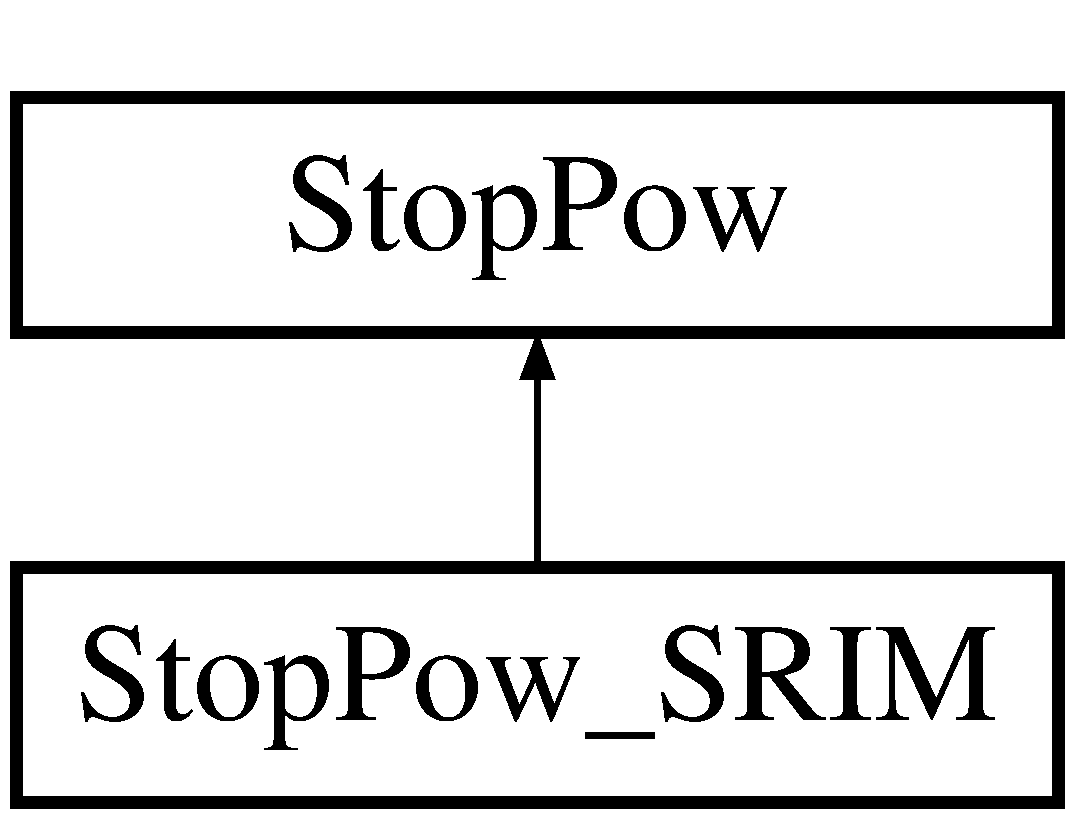
\includegraphics[height=2.000000cm]{class_stop_pow___s_r_i_m}
\end{center}
\end{figure}
\subsection*{Public Member Functions}
\begin{DoxyCompactItemize}
\item 
\hyperlink{class_stop_pow___s_r_i_m_ab901771706e85a82531b0be9b01642b5}{Stop\-Pow\-\_\-\-S\-R\-I\-M} (string fname)
\item 
\hyperlink{class_stop_pow___s_r_i_m_a62aef1b8aee5d00c49e9bc04ef891a2d}{$\sim$\-Stop\-Pow\-\_\-\-S\-R\-I\-M} ()
\item 
float \hyperlink{class_stop_pow___s_r_i_m_a762011aa6430e95dc3e06bf8d5791b05}{d\-Edx\-\_\-\-Me\-V\-\_\-um} (float E)
\item 
float \hyperlink{class_stop_pow___s_r_i_m_acd593e878322cc5e65649c2346242188}{d\-Edx\-\_\-\-Me\-V\-\_\-mgcm2} (float E)
\end{DoxyCompactItemize}
\subsection*{Additional Inherited Members}


\subsection{Detailed Description}
Cold-\/matter tabulated stopping. 

A wrapper class for calculating stopping powers using tabulated S\-R\-I\-M data (stored in csv files) Linear interpolation is performed between data points.

\begin{DoxyAuthor}{Author}
Alex Zylstra 
\end{DoxyAuthor}
\begin{DoxyDate}{Date}
2013/03/29 
\end{DoxyDate}


\subsection{Constructor \& Destructor Documentation}
\hypertarget{class_stop_pow___s_r_i_m_ab901771706e85a82531b0be9b01642b5}{\index{Stop\-Pow\-\_\-\-S\-R\-I\-M@{Stop\-Pow\-\_\-\-S\-R\-I\-M}!Stop\-Pow\-\_\-\-S\-R\-I\-M@{Stop\-Pow\-\_\-\-S\-R\-I\-M}}
\index{Stop\-Pow\-\_\-\-S\-R\-I\-M@{Stop\-Pow\-\_\-\-S\-R\-I\-M}!StopPow_SRIM@{Stop\-Pow\-\_\-\-S\-R\-I\-M}}
\subsubsection[{Stop\-Pow\-\_\-\-S\-R\-I\-M}]{\setlength{\rightskip}{0pt plus 5cm}Stop\-Pow\-\_\-\-S\-R\-I\-M\-::\-Stop\-Pow\-\_\-\-S\-R\-I\-M (
\begin{DoxyParamCaption}
\item[{string}]{fname}
\end{DoxyParamCaption}
)}}\label{class_stop_pow___s_r_i_m_ab901771706e85a82531b0be9b01642b5}
Constructor for S\-R\-I\-M object. Data file must be in standard S\-R\-I\-M format. 
\begin{DoxyParams}{Parameters}
{\em fname} & file name (or relative path) for the data \\
\hline
\end{DoxyParams}

\begin{DoxyExceptions}{Exceptions}
{\em ios\-\_\-base\-::failure} & \\
\hline
\end{DoxyExceptions}
\hypertarget{class_stop_pow___s_r_i_m_a62aef1b8aee5d00c49e9bc04ef891a2d}{\index{Stop\-Pow\-\_\-\-S\-R\-I\-M@{Stop\-Pow\-\_\-\-S\-R\-I\-M}!$\sim$\-Stop\-Pow\-\_\-\-S\-R\-I\-M@{$\sim$\-Stop\-Pow\-\_\-\-S\-R\-I\-M}}
\index{$\sim$\-Stop\-Pow\-\_\-\-S\-R\-I\-M@{$\sim$\-Stop\-Pow\-\_\-\-S\-R\-I\-M}!StopPow_SRIM@{Stop\-Pow\-\_\-\-S\-R\-I\-M}}
\subsubsection[{$\sim$\-Stop\-Pow\-\_\-\-S\-R\-I\-M}]{\setlength{\rightskip}{0pt plus 5cm}Stop\-Pow\-\_\-\-S\-R\-I\-M\-::$\sim$\-Stop\-Pow\-\_\-\-S\-R\-I\-M (
\begin{DoxyParamCaption}
{}
\end{DoxyParamCaption}
)}}\label{class_stop_pow___s_r_i_m_a62aef1b8aee5d00c49e9bc04ef891a2d}
Destructor 

\subsection{Member Function Documentation}
\hypertarget{class_stop_pow___s_r_i_m_acd593e878322cc5e65649c2346242188}{\index{Stop\-Pow\-\_\-\-S\-R\-I\-M@{Stop\-Pow\-\_\-\-S\-R\-I\-M}!d\-Edx\-\_\-\-Me\-V\-\_\-mgcm2@{d\-Edx\-\_\-\-Me\-V\-\_\-mgcm2}}
\index{d\-Edx\-\_\-\-Me\-V\-\_\-mgcm2@{d\-Edx\-\_\-\-Me\-V\-\_\-mgcm2}!StopPow_SRIM@{Stop\-Pow\-\_\-\-S\-R\-I\-M}}
\subsubsection[{d\-Edx\-\_\-\-Me\-V\-\_\-mgcm2}]{\setlength{\rightskip}{0pt plus 5cm}float Stop\-Pow\-\_\-\-S\-R\-I\-M\-::d\-Edx\-\_\-\-Me\-V\-\_\-mgcm2 (
\begin{DoxyParamCaption}
\item[{float}]{E}
\end{DoxyParamCaption}
)\hspace{0.3cm}{\ttfamily [virtual]}}}\label{class_stop_pow___s_r_i_m_acd593e878322cc5e65649c2346242188}
Get stopping power from the data. 
\begin{DoxyParams}{Parameters}
{\em E} & the particle energy in Me\-V \\
\hline
\end{DoxyParams}
\begin{DoxyReturn}{Returns}
d\-E/dx in Me\-V/(mg/cm2) 
\end{DoxyReturn}

\begin{DoxyExceptions}{Exceptions}
{\em invalid\-\_\-argument} & \\
\hline
\end{DoxyExceptions}


Implements \hyperlink{class_stop_pow}{Stop\-Pow}.

\hypertarget{class_stop_pow___s_r_i_m_a762011aa6430e95dc3e06bf8d5791b05}{\index{Stop\-Pow\-\_\-\-S\-R\-I\-M@{Stop\-Pow\-\_\-\-S\-R\-I\-M}!d\-Edx\-\_\-\-Me\-V\-\_\-um@{d\-Edx\-\_\-\-Me\-V\-\_\-um}}
\index{d\-Edx\-\_\-\-Me\-V\-\_\-um@{d\-Edx\-\_\-\-Me\-V\-\_\-um}!StopPow_SRIM@{Stop\-Pow\-\_\-\-S\-R\-I\-M}}
\subsubsection[{d\-Edx\-\_\-\-Me\-V\-\_\-um}]{\setlength{\rightskip}{0pt plus 5cm}float Stop\-Pow\-\_\-\-S\-R\-I\-M\-::d\-Edx\-\_\-\-Me\-V\-\_\-um (
\begin{DoxyParamCaption}
\item[{float}]{E}
\end{DoxyParamCaption}
)\hspace{0.3cm}{\ttfamily [virtual]}}}\label{class_stop_pow___s_r_i_m_a762011aa6430e95dc3e06bf8d5791b05}
Get stopping power from the data. 
\begin{DoxyParams}{Parameters}
{\em E} & the particle energy in Me\-V \\
\hline
\end{DoxyParams}
\begin{DoxyReturn}{Returns}
d\-E/dx in Me\-V/um 
\end{DoxyReturn}

\begin{DoxyExceptions}{Exceptions}
{\em invalid\-\_\-argument} & \\
\hline
\end{DoxyExceptions}


Implements \hyperlink{class_stop_pow}{Stop\-Pow}.



The documentation for this class was generated from the following file\-:\begin{DoxyCompactItemize}
\item 
/\-Users/alex/\-Dropbox/\-Research/workspace/\-Stop\-Pow/src/Stop\-Pow\-\_\-\-S\-R\-I\-M.\-h\end{DoxyCompactItemize}

\addcontentsline{toc}{part}{Index}
\printindex
\end{document}
